% !TEX program = lualatex
\documentclass[aspectratio=43,professionalfonts,handout]{beamer}
\usepackage{beamer_template}

\newcommand{\LectureNum}{01}
\newcommand{\LectureTitle}{関数とグラフ}
\newcommand{\TextPages}{p.\,72-75}
\newcommand{\NextTopic}{２次関数のグラフ（１）}
\newcommand{\NextPages}{p.\,75-77}
\newcommand{\CourseName}{基礎数学B}
\renewcommand{\TermName}{前期}

\begin{document}

% -----------------------------------------------
% スライド1: 表紙＋目標＋用語・定義
% -----------------------------------------------
\begin{frame}{\CourseName\quad 第\LectureNum 回「\LectureTitle 」}
  {\small \TermName\quad \TeacherName\quad ／\quad 教科書 \TextPages\quad
  \textbf{目標}：関数の概念・定義域・値域を理解し、1次関数のグラフが描ける}

  \begin{block}{用語・定義}
  \begin{description}[labelwidth=5.5em]
    \item[\kw{関数}] ~
    \item[\kw{独立変数}] ~
    \item[\kw{従属変数}] ~
    \item[\kw{定義域}] ~
    \item[\kw{値域}] ~
    \item[\kw{f(a)}] ~
  \end{description}
  \end{block}
\end{frame}

% -----------------------------------------------
% スライド2: 公式・性質
% -----------------------------------------------
\begin{frame}{公式・性質}
  \begin{block}{}
  \begin{itemize}
    \item 1次関数 y=ax+b
    \item 定数関数 y=c
    \item x=d（垂直な直線）
  \end{itemize}
  \end{block}
\end{frame}

% -----------------------------------------------
% スライド3: 図・グラフ（TikZコードを手動追加）
% -----------------------------------------------
\begin{frame}{図・グラフ}
  \centering
  % TODO: 座標平面と象限; y=x+1、y=2、x=-1 のグラフ
  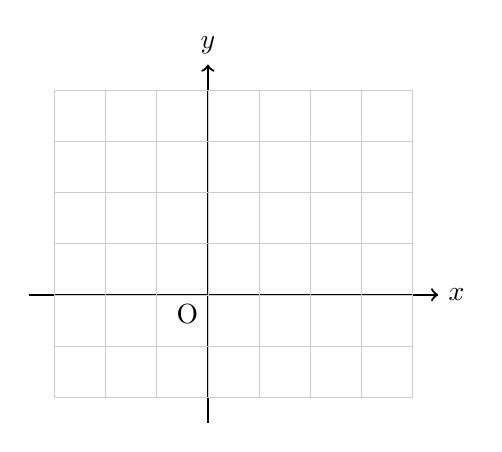
\begin{tikzpicture}[scale=0.65]
    \draw[->,thick] (-3.5,0) -- (4.5,0) node[right]{$x$};
    \draw[->,thick] (0,-2.5) -- (0,4.5) node[above]{$y$};
    \node[below left] at (0,0) {O};
    \draw[gray!40, very thin] (-3,-2) grid (4,4);
    % ここにグラフを描画
  \end{tikzpicture}
\end{frame}

% -----------------------------------------------
% スライド4: 例1→問1
% -----------------------------------------------
\begin{frame}{例1→問1}
  \begin{exampleblock}{例1) p.73}
    （板書で解説）
  \end{exampleblock}

  \vfill

  \begin{block}{問1) p.73\quad 自分で解いてみよう}
    （ノートに解くこと）
  \end{block}
\end{frame}

% -----------------------------------------------
% スライド5: 例2→問2
% -----------------------------------------------
\begin{frame}{例2→問2}
  \begin{exampleblock}{例2) p.74}
    （板書で解説）
  \end{exampleblock}

  \vfill

  \begin{block}{問2) p.74\quad 自分で解いてみよう}
    （ノートに解くこと）
  \end{block}
\end{frame}

% -----------------------------------------------
% まとめ
% -----------------------------------------------
\begin{frame}{まとめ}
  \begin{itemize}
    \item 関数とは x の値に y がただ1つ対応する関係
    \item 定義域は x の範囲、値域は y の範囲
    \item 1次関数 y=ax+b のグラフは傾き a・切片 b の直線
    \item f(a+h) ≠ f(a)+h に注意
  \end{itemize}

  \vfill
  {\small 基本問題：143, 144}
\end{frame}

\end{document}
